% Created 2015-11-19 Thu 15:51
\documentclass[a4paper]{tufte-handout}
\usepackage[scaled=0.95]{roboto}
\usepackage{mathpazo}
\linespread{1.05}
\usepackage{eulervm}
\usepackage[usenames]{xcolor}


%% footnote color 
\renewcommand{\thefootnote}{\textcolor{Gray}{\arabic{footnote}}}
\makeatletter

\renewcommand\@footnotetext[2][0pt]{%
  \marginpar{%
    \hbox{}\vspace*{#1}%
    \def\baselinestretch {\setspace@singlespace}%
    \reset@font\footnotesize%
    \@tufte@margin@par% use parindent and parskip settings for marginal text
    \vspace*{-1\baselineskip}\noindent%
    \protected@edef\@currentlabel{%
       \csname p@footnote\endcsname\@thefnmark%
    }%
    \color{Gray}
    \color@begingroup%
       \@makefntext{%
         \ignorespaces#2%
       }%
    \color@endgroup%
  }%
}%

\makeatother
%%==============================================================================
%%                                 SECTIONS
%%==============================================================================
%% section numbering to subsection
\setcounter{secnumdepth}{2}
\renewcommand{\thesection}{\Roman{section}}
\renewcommand{\thesubsection}{\thesection.\Alph{subsection}}
\renewcommand{\thesubsubsection}{\thesubsection\arabic{subsubsection})}
\renewcommand{\theparagraph}{\roman{paragraph}}
 
%%==============================================================================
%%                                 COLORS
%%==============================================================================
%% section format
\titleformat{\section}%
  {\normalfont\Huge\color{Cerulean}}% format applied to label+text
  {\llap{\colorbox{Cerulean}{\parbox{1.5cm}{\hfill\color{white}\thesection}}}}% label
  {1em}% horizontal separation between label and title body
  {}% before the title body
  []% after the title body

% subsection format
\titleformat{\subsection}%
  {\normalfont\Large\itshape\color{TealBlue}}% format applied to label+text
  {\llap{\colorbox{TealBlue}{\parbox{1cm}{\hfill\color{white}\thesubsection}}}}% label
  {0.5em}% horizontal separation between label and title body
  {}% before the title body
  []% after the title body

\renewcommand{\footnotesize}{\scriptsize}
\setcaptionfont{\color{Gray}\footnotesize}
\setsidenotefont{\color{Gray}\footnotesize}
\setmarginnotefont{\color{Gray}\itshape\footnotesize}

\usepackage[utf8]{inputenc}
\usepackage[T1]{fontenc}
\usepackage{graphicx}
\usepackage{longtable}
\usepackage{float}
\usepackage{hyperref}
\usepackage{wrapfig}
\usepackage{rotating}
\usepackage[normalem]{ulem}
\usepackage{amsmath}
\usepackage{textcomp}
\usepackage{marvosym}
\usepackage{wasysym}
\usepackage{amssymb}
\usepackage[scaled=0.9]{zi4}
\usepackage[usenames, dvipsnames]{xcolor}
\usepackage[protrusion=true, expansion=alltext, tracking=true, kerning=true]{microtype}
\usepackage{siunitx}
\usepackage[frenchle, frenchb]{babel}
\usepackage[euler-digits]{eulervm}
\renewcommand{\footnotesize}{\small}
\author{Samuel BARRETO}
\date{\today}
\title{Premières Analyses des Données de Séquençage}
\hypersetup{
 pdfauthor={Samuel BARRETO},
 pdftitle={Premières Analyses des Données de Séquençage},
 pdfkeywords={},
 pdfsubject={},
 pdfcreator={Emacs 24.5.1 (Org mode 8.3.2)}, 
 pdflang={Frenchb}}
\begin{document}

\maketitle

\section{Qualité des données}
\label{sec:orgheadline5}
\subsection{qualité du séquençage}
\label{sec:orgheadline1}
\begin{marginfigure}
  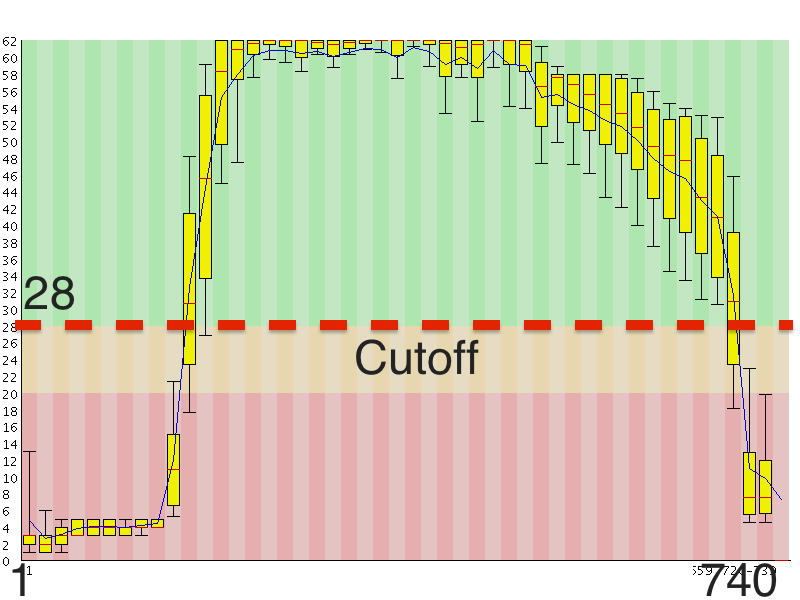
\includegraphics[width=\linewidth]{../untrimmed.png}
  \caption{Qualité des séquences \emph{avant} d'être trimmées et filtrées
      sur la qualité}
\end{marginfigure}

\begin{marginfigure}
  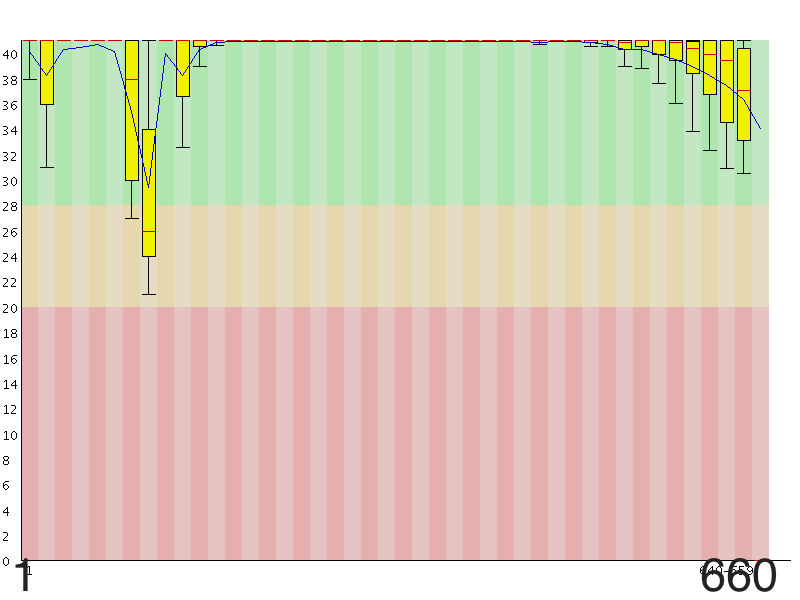
\includegraphics[width=\linewidth]{../trimmed.png}
  \caption{Qualité des séquences \emph{après} avoir été trimmées et filtrées
      sur la qualité}
\end{marginfigure}
Globalement la plupart des séquences était de bonne qualité. Sur les \(192\)
envoyées à séquencer, \(179\) ont été retenues pour l'analyse, soit 93\%.

Étant donnée la faible qualité des bases en début et en fin de séquence, elles
ont été tronquées. Le score \(28\) semblait le seuil naturel de qualité. De plus,
toutes les séquences qui avaient une longueur inférieure à \(620\) étaient
généralement mal alignées. Elles ont été éliminées de l'analyse. 

\subsection{Présence de contaminations ?}
\label{sec:orgheadline2}
Pas évident à déterminer : voir après. 
\subsection{Observations générales}
\label{sec:orgheadline3}

\begin{center}
\small
\begin{tabular}{cccc}
\toprule
\textbf{nombre de SNP par} &  &  & \\
\textbf{gene synthétique} & \textbf{moyen} & \textbf{sd} & \textbf{median}\\
\midrule
global & 14.4 & 6.4 & 15.0\\
strong & 15.5 & 6.2 & 15.5\\
weak & 13.3 & 6.5 & 13.0\\
\bottomrule
\end{tabular}
\end{center}

\subsection{Nombre de SNPs}
\label{sec:orgheadline4}

\begin{center}
\small
\begin{tabular}{ccc}
\toprule
 & \textbf{strong} & \textbf{weak}\\
\midrule
nombre de SNP par gène synthétique & 1337 & 1162\\
nombre de substitutions & \textbf{1970} & 529\\
\bottomrule
\end{tabular}
\end{center}

Pour un nombre de SNPs par gène synthétique sensiblement équivalent, il y a
\(3.7\) fois plus de substitutions \emph{strong} que \emph{weak} !

\begin{marginfigure}
  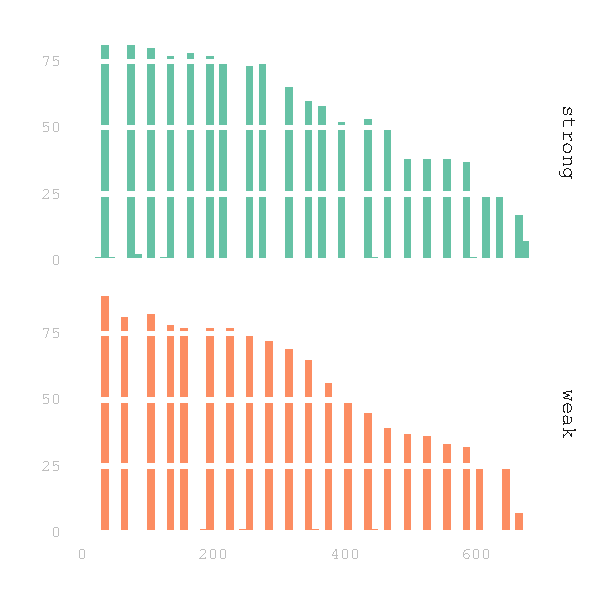
\includegraphics[width=\linewidth]{../strong_vs_weak.pdf}
  \caption{Distribution du nombre de substitutions de type \emph{strong,} comparée à
    celles de type \emph{weak.} }
\end{marginfigure}

\newpage
\section{Distribution des SNPs}
\label{sec:orgheadline8}
\subsection{Distribution globale}
\label{sec:orgheadline6}
\begin{figure*}[h]
  \centering
  \includegraphics[width=\linewidth]{../snp_distribution.pdf}
  \caption{La distibution des SNPs, sans tenir compte de la qualité de la
    mutation. La couleur représente le mutant d'origine, qu'il soit sensé être
    Weak ou Strong.}
  \label{figure1}
\end{figure*}

Ce graphe représente la distribution des SNPs sur la séquence de référence. Les
barres vertes représentent les SNP des gènes synthétiques Strong, les rouges
celles des Weak. 

Première observation : il y a plus de SNP dans les régions 5' que 3'. Artefact
de séquençage ? Quand on regarde la qualité du \emph{base call} et les spectrogrammes
associés, il ne semble pas. 

Deuxième observation : les gènes synthétiques Strong génèrent plus de SNPs en 3'
que les Weak. À tester, pas certain que ce soit significatif. 

Troisème observation : malgré les filtres et le tronquage, il reste du bruit.
Quelques SNP ne sont pas à leur place attendue. Pas facile à éliminer…

\newthought{Conclusion} : il y a plus de substitutions dans les régions 3' que 5',
sur la fin de la conversion tract. Où se fait le switch ? 

\marginnote{ À noter qu'on n'a pas de SNP après la position 691, alors que la
  séquence de référence mesure $734$bp. C'est dû au \emph{trimming} des
  séquences. On perd l'information des premiers SNP. }

\newpage
\subsection{Distribution de la qualité des mutation}
\label{sec:orgheadline7}

\begin{figure*}[h]
  \centering
  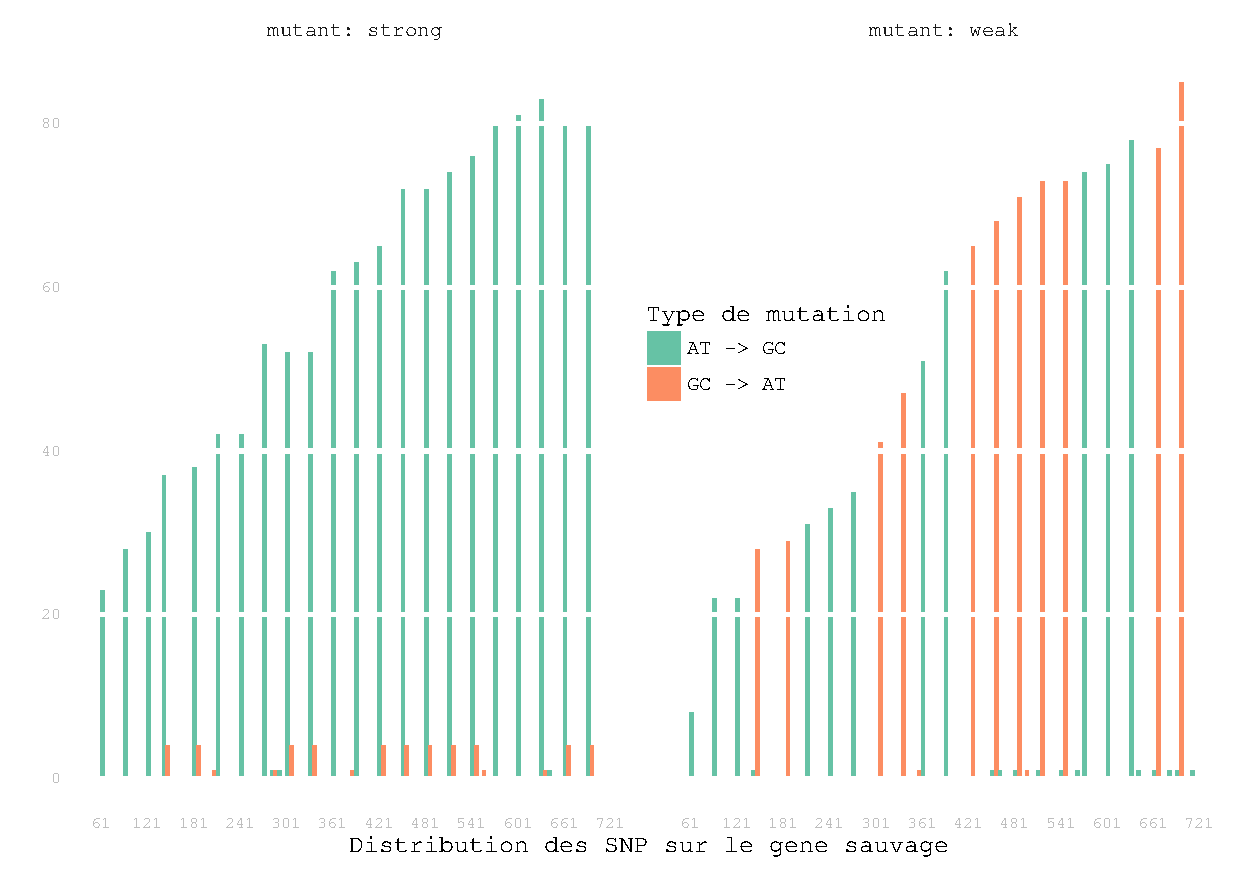
\includegraphics[width=\linewidth]{../substitution_distribution.pdf}
  \caption{\textbf{Distribution des SNP par position sur la séquence de référence.} \\
  On retrouve bien les positions des polymorphismes ``artificiels'', toutes les
  $30$ paires de bases. En vert les mutations \emph{strong} et en rouge les
  mutations \emph{weak}. Les mutants Strong montrent exclusivement des
  substitutions \emph{strong}. Les mutants Weak montrent cependant des
  choses différentes. Il y a beaucoup de mutations \emph{strong}, contrairement
  à l'attendu. 
  }
  \label{figure2}
\end{figure*}

Ce graphe montre un résultat surprenant. 

À gauche, la distribution des SNP générés par les gènes synthétiques de type
Strong ; à droite, celle des gènes synthétiques de type Weak. Les barres vertes
représentent les substitutions vers \(GC\), \emph{strong} ; les barres rouges les
substitutions vers \(AT\), \emph{weak}.

Lorsque le gène synthétique est de type Strong, les substitutions occasionnées
sont --- quasiment --- exclusivement de type \emph{strong}.

Mais lorsque le gène synthétique est de type Weak, les substitutions
occasionnées sont à la fois de type \emph{weak} et de type \emph{strong}. Les positions
particulièrement concernées sont celles autour de \(60\), \(240\), \(420\) et \(600\)
bp.

\newpage
\newthought{Montré autrement}, on voit le problème plus clairement.  


\begin{figure*}[h]
  \centering
  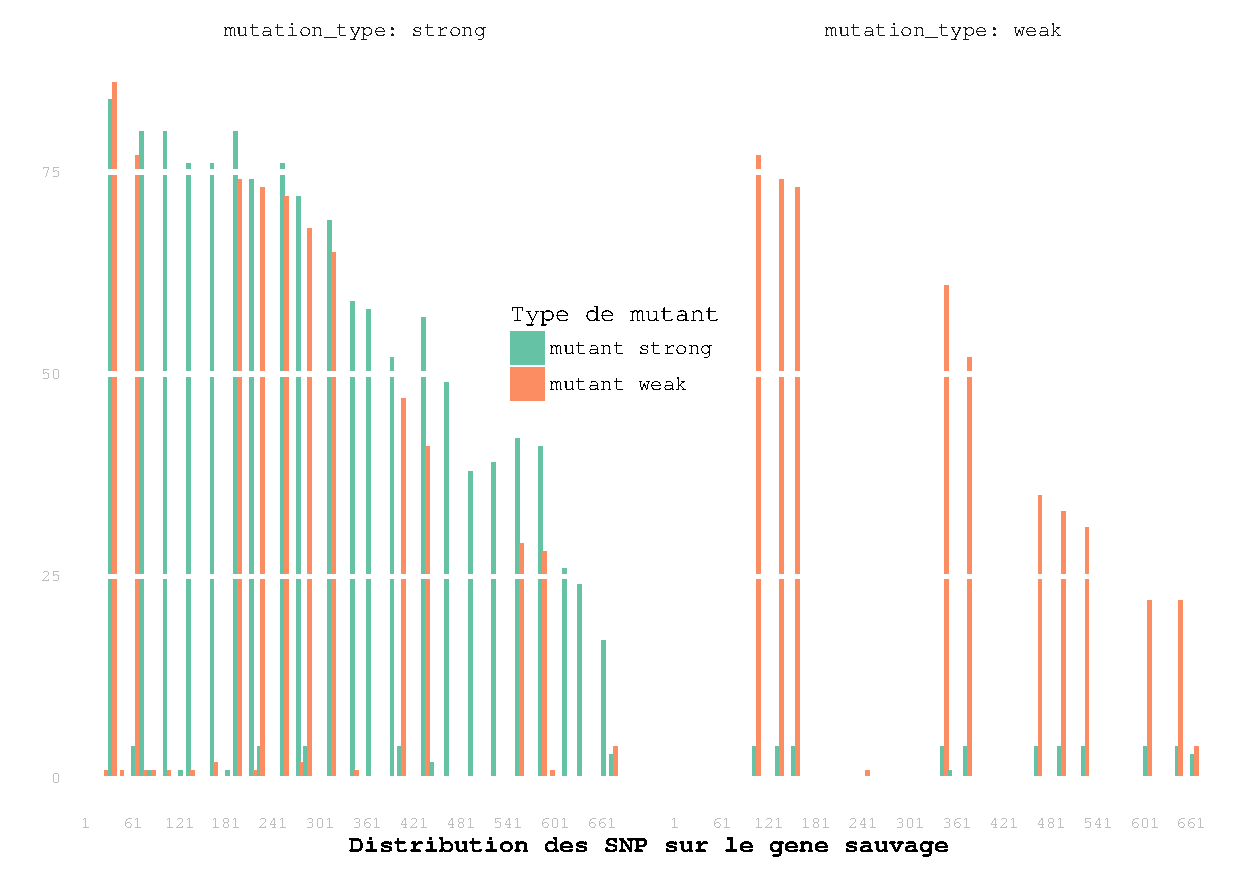
\includegraphics[width=\linewidth]{../muttype_plot.pdf}
  \caption{\textbf{Distribution de la qualité des substitutions}. \\
    À gauche la distribution des substitutions vers $GC$, à droite celle des
    substitutions vers $A$ ou $T$. On voit bien que les mutations \emph{weak} sont
    quasiment exclusivement dans les mutants de type Weak, alors qu'on retrouve
    des mutations \emph{strong} dans les deux types de mutants.}
  \label{figure3}
\end{figure*}

\begin{marginfigure}[5in]
  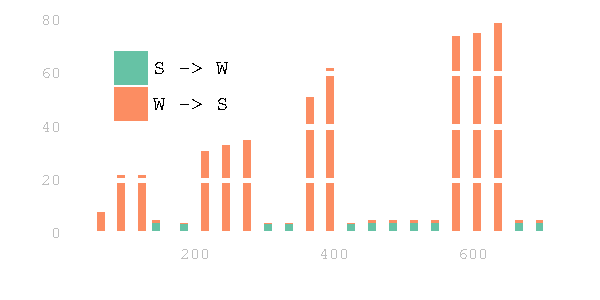
\includegraphics[width=\linewidth]{../outliers.pdf}
  \caption{Avec ici un focus sur les \em{outliers} qui n'en sont pas}
  \label{figure7}
\end{marginfigure}

À gauche, la distribution des substitutions de type \emph{strong}, vers \(GC\). À droite,
celle des substitutions de type \emph{weak}, vers \(AT\). Les barres vertes
représentent les substitutions générés par les gènes synthétiques Strong, les
rouges celles des Weak. 

En figure \ref{figure7}, la distribution de ces SNP qui ne devraient pas
exister : les substitutions \emph{strong} générées par les mutants Weak --- en rouge
---, et les substitutions \emph{weak} générées par les mutants Strong --- en vert
---. Trois graphes pour dire la même chose. 

\newthought{Conclusion} : seuls les gènes synthétiques Weak génèrent des
substitutions \emph{weak}. Les substitutions \emph{strong} sont générées à la fois par les
gènes synthétiques Strong et par les Weak.


\clearpage
\section{Distribution de la position de basculement}
\label{sec:orgheadline11}
\subsection{Basculement terminal global}
\label{sec:orgheadline9}
\begin{figure}
  \centering
  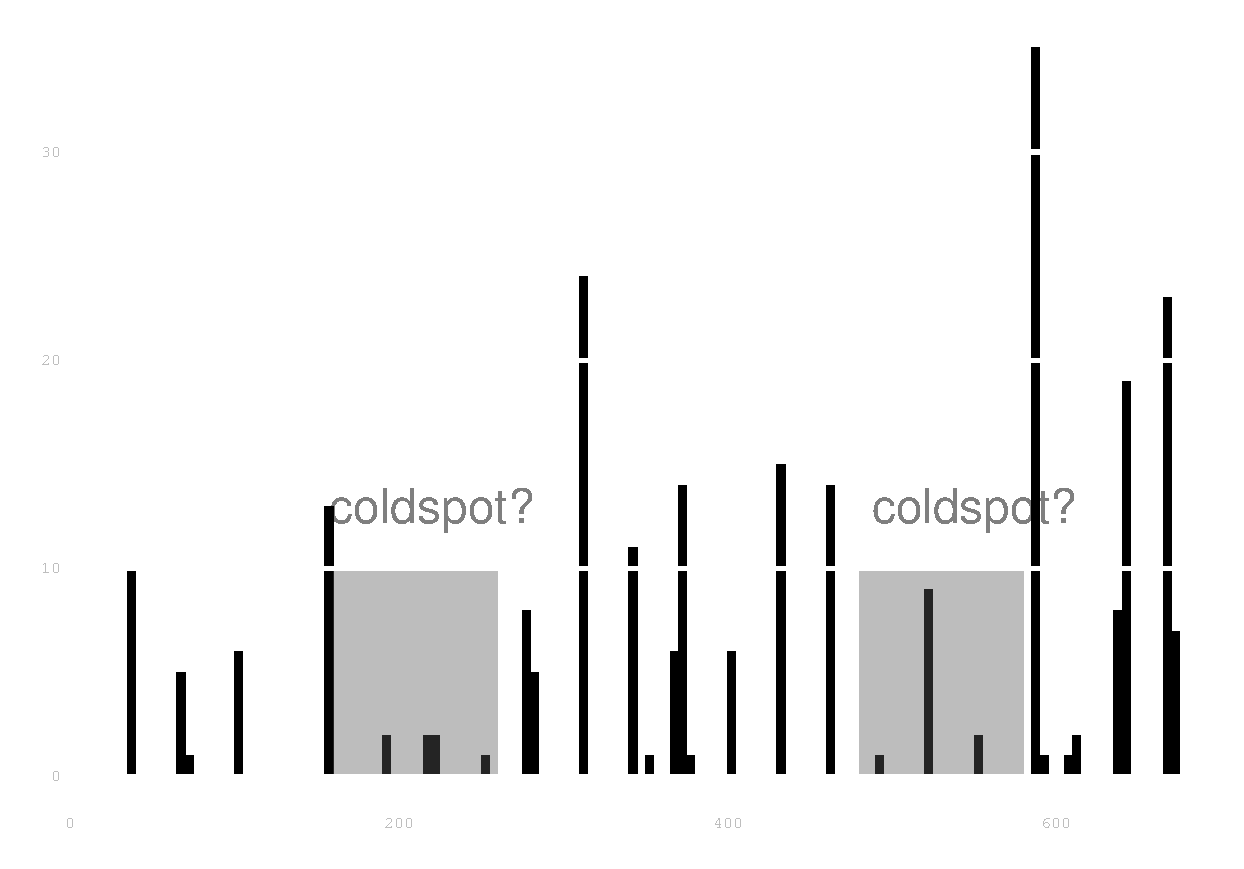
\includegraphics[width=\linewidth]{../switch_position_globale.pdf}
  \caption{\textbf{Position des switch, indifféremment de la qualité de la
      substition ou du mutant}. \\
    Il y a des disparités dans la distribution des positions de basculement. Il
    y a beaucoup de basculement dès le début, moins vers la fin. Il semble y
    avoir une sorte de \emph{coldspot} local, autour de $500$bp et $200$bp sur
    la séquence de référence. }
\end{figure}

Ce graphe représente la distribution du dernier SNP par mutant : autrement dit,
la position de basculement. 

Il y a une très forte hétérogénéité : la distribution est clairement
multi-modale. Peut-on parler de coldspot / hotspot local ?

\newpage
\subsection{Position terminale de basculement par type de mutation}
\label{sec:orgheadline10}

\begin{figure*}
  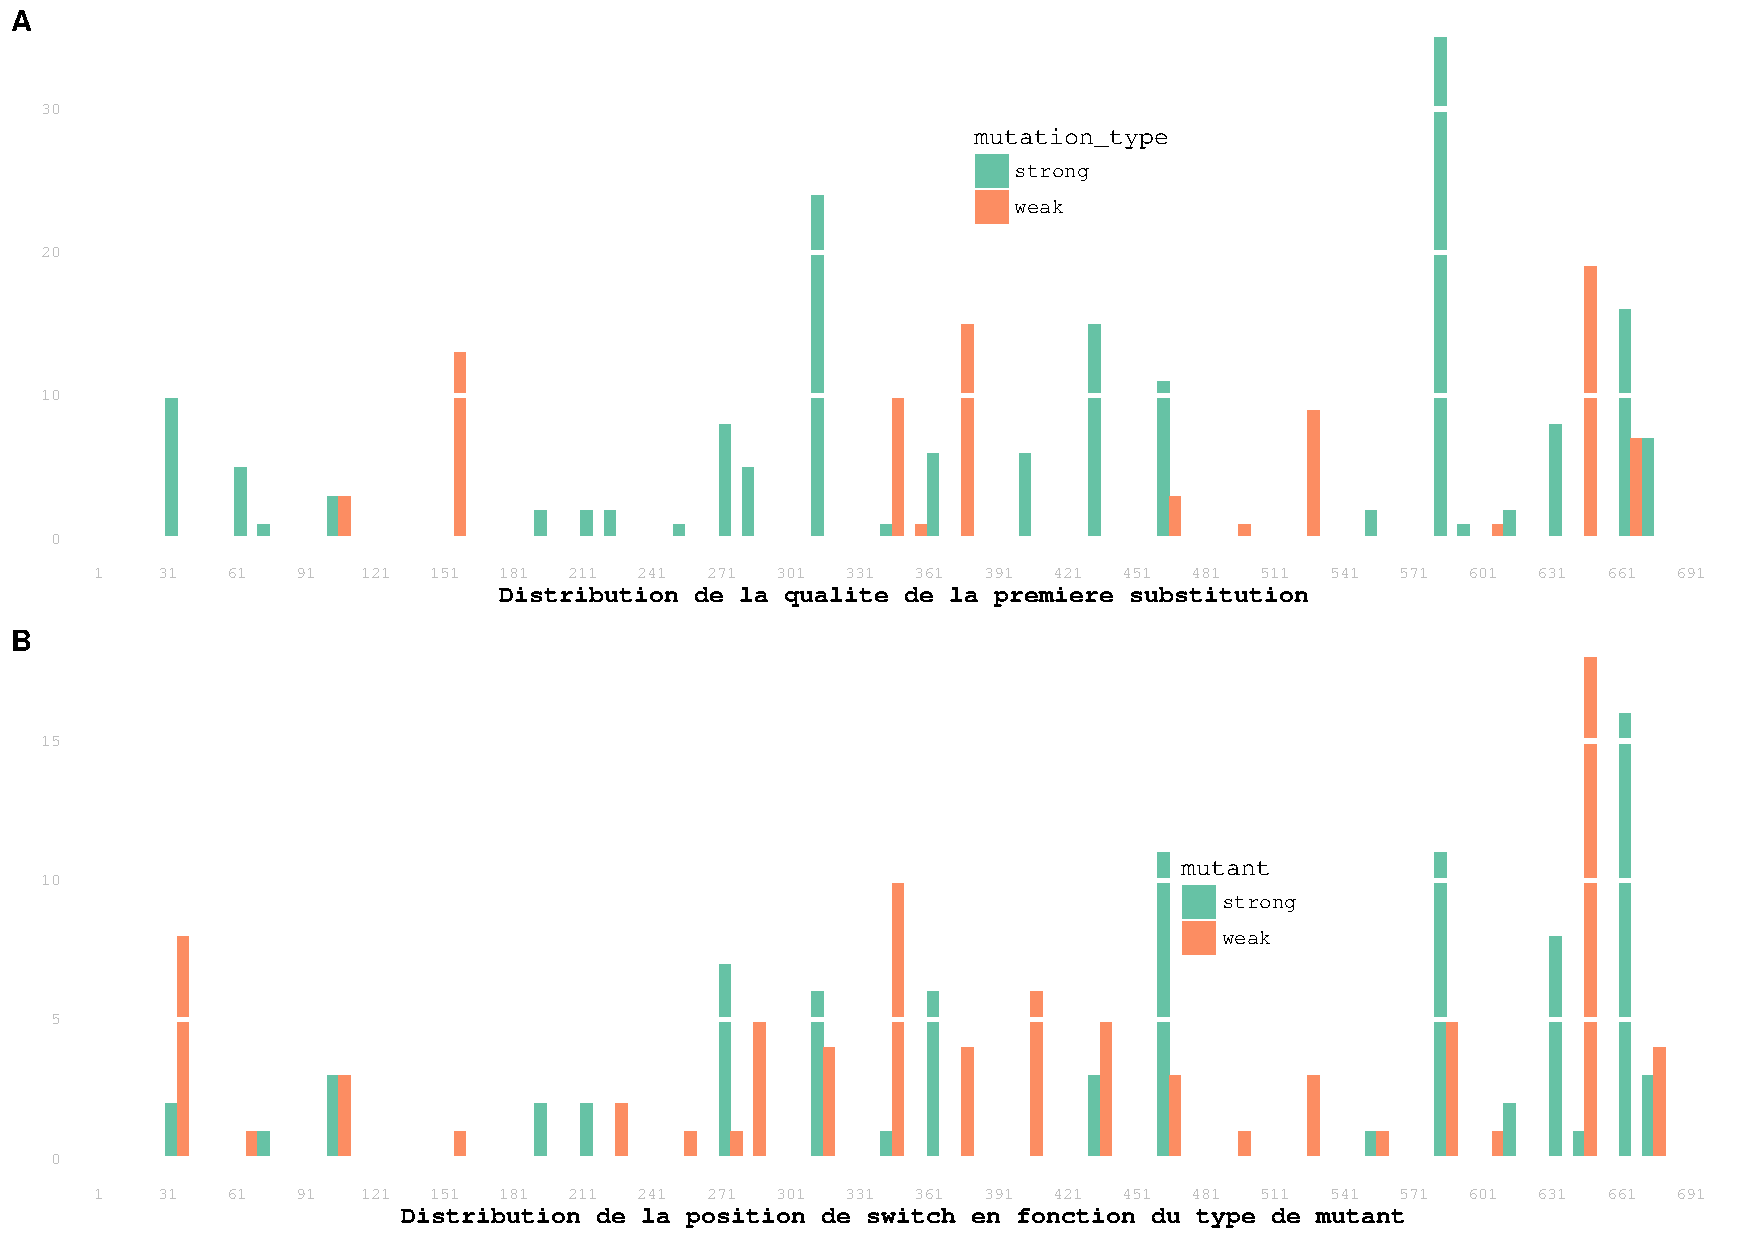
\includegraphics[width=\linewidth]{../switch_pos_by_mutant.pdf}
  \caption{Position des switch en fonction du type de mutant. \\
    Le graphe \texttt{A} représente la distribution et la qualité du premier
    SNP, $AT \mapsto GC$ est \emph{strong} et $GC \mapsto AT$ est \emph{weak}.
    Le graphe \texttt{B} représente la distribution du premier SNP par clone, en
    fonction de la qualité du clone, Strong ou Weak. \\
    On ne semble pas voir de différence significative. Dans les deux cas, les
    distributions sont assez similaires pour le \emph{weak} et le \emph{strong}.
    Cependant, des différences existent entre les graphes \texttt{A} et
    \texttt{B} : toutes les premières substitutions sont de type
    \emph{strong.} \\
    Il y a toujours le même patron de coldspot autour de 541bp.}
\end{figure*}

Le graphe \texttt{A} a été obtenu en filtrant le jeu de donnée de la façon suivante : 
\begin{itemize}
\item groupe par clone et par type de mutation.
\item demande la première position de SNP ``groupwise''.
\end{itemize}
Il représente la position du dernier SNP de type \emph{strong} ou \emph{weak}, par gène
synthétique. En fait il ne veut pas dire grand chose mais j'ai pas eu le temps
de l'enlever…

Le graphe \texttt{B} a été obtenu en filtrant le jeu de donnée de la façon suivante :
\begin{itemize}
\item groupe par clone
\item demande la première position de SNP ``groupwise''.
\end{itemize}
Il représente la position du dernier SNP par type de gène synthétique. Il
correspond au graphe de Vincent en figure \ref{figvincent}. 

\newpage

\newthought{À vue d'œil}, il n'y a pas de variation significative sur la
distribution des SNPs, quelle que soit la qualité du gène synthétique ou de la
substitution.

\begin{marginfigure}
  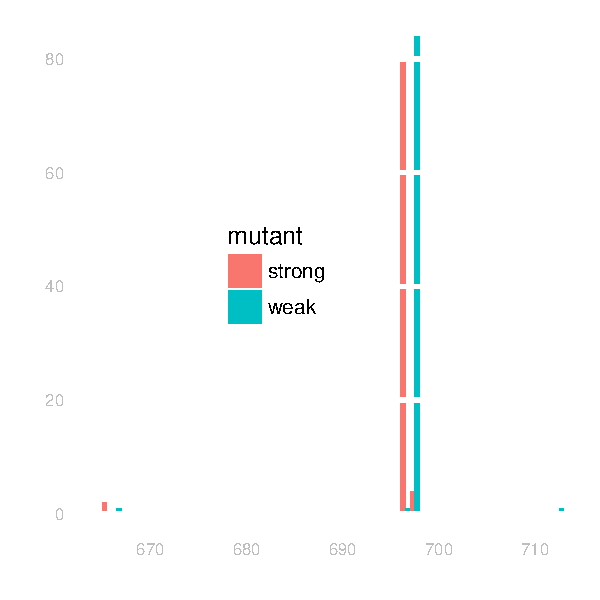
\includegraphics[width=\linewidth]{../end_switch.pdf}
  \caption{Position du premier SNP.\\
    Pas de variation là dessus. À priori les deux mutants terminent au même
    endroit, c'est à dire au premier site avant le cutoff de trimming. 
  }
\end{marginfigure}


\begin{marginfigure}
  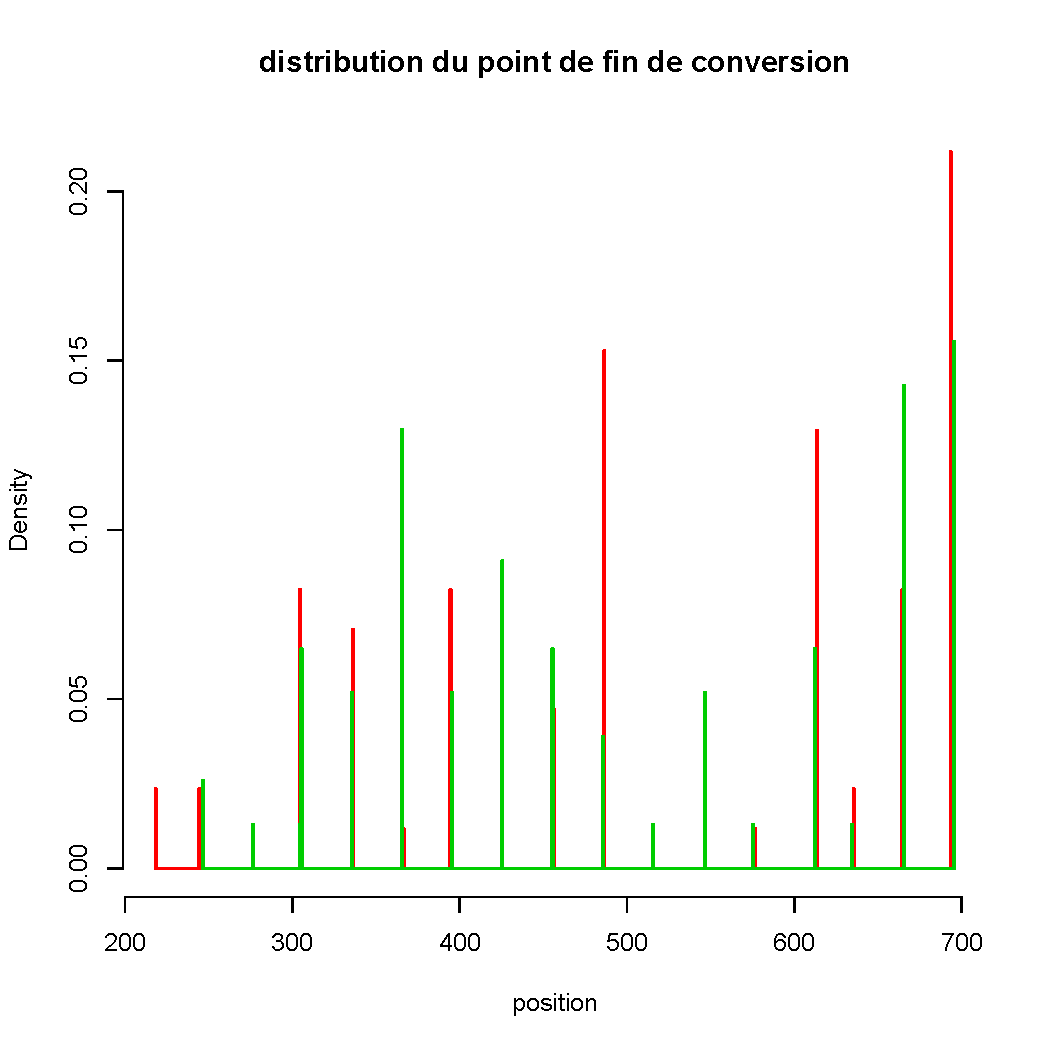
\includegraphics[width=\linewidth]{../vincent_plot.pdf}
  \caption{Position du dernier SNP.
  }
  \label{figvincent}
\end{marginfigure}
\end{document}